W niniejszej pracy został opisany proces przygotowania systemu wybudowanego opartego na koncepcji Internet of Things.
Przedstawiono narzędzia umożliwiające zaprojektowanie, i wytworzenie takiego systemu, wraz z wyjaśnieniem decyzji podejmowanych przy wyborze poszczególnych. Opisane zostały również wybrane koncepcje wytwarzania oprogramowania i oraz autorska metoda synchronizacji danych przy użyciu asynchronicznych zapytań RESTowych oraz obiektów JSON.

Część praktyczna pracy składa się z urządzenia odpowiednio skonfigurowanego do pracy z wyświetlaczem dotykowym, aplikacji mobilnej, która  łączy w sobie wszystkie założone funkcjonalności takie jak możliwość dodawania i zarządzania listami zadań, możliwością porządkowania zadań według priorytetów oraz sterowanie wykonywaniem zadań (czasomierz). Zaimplementowany został mechanizm synchronizacji oraz aplikacja webowa. Całość tworzy system, który dowodzi spełnienia postawionych założeń oraz prezentuje przykładowe zastosowanie systemu z użyciem platformy mikroprocesorowej - w tym przypadku - systemu wspomagającego zarządzaniem czasem i zadaniami.

Podczas projektowania systemu autorzy nie przewidzieli, że zastosowane rozwiązanie - zestaw bibliotek Kivy obsługujące część graficzną aplikacji - nie będzie odbsługiwane przez wbudowaną w urządzenie (Raspberry Pi) kartę graficzną. Bez wspomagania sprzętowego aplikacja działa bardzo wolno. W najnowszym wydaniu, producent Kivy zapowiedział wsparcie dla tego urządzenia.

Podsumowując, współczesna technologia umożliwia tworzenie oprogramowania użytkowego, które może w pełni integrować się z istniejącymi systemami wbudowanymi takimi jak składowe iteligentnego domu, czy urządzeń zaprojektowanych według koncepcji Internet of Things. Stworzenie systemu rozproszonego według opisanego w pracy rozwiązania wymaga niewielkiego nakładu finansowego i czasowego. Spektrum rozwiązań jakie podobne systemy mogą oferować, jest bardzo duże i zróżnicowane, podobnie jak to ma miejsce w przypadku aplikacji mobilnych dedykowanych dla wybranych producentów systemów operacyjnych.

\begin{figure}[ht]
  \centering
  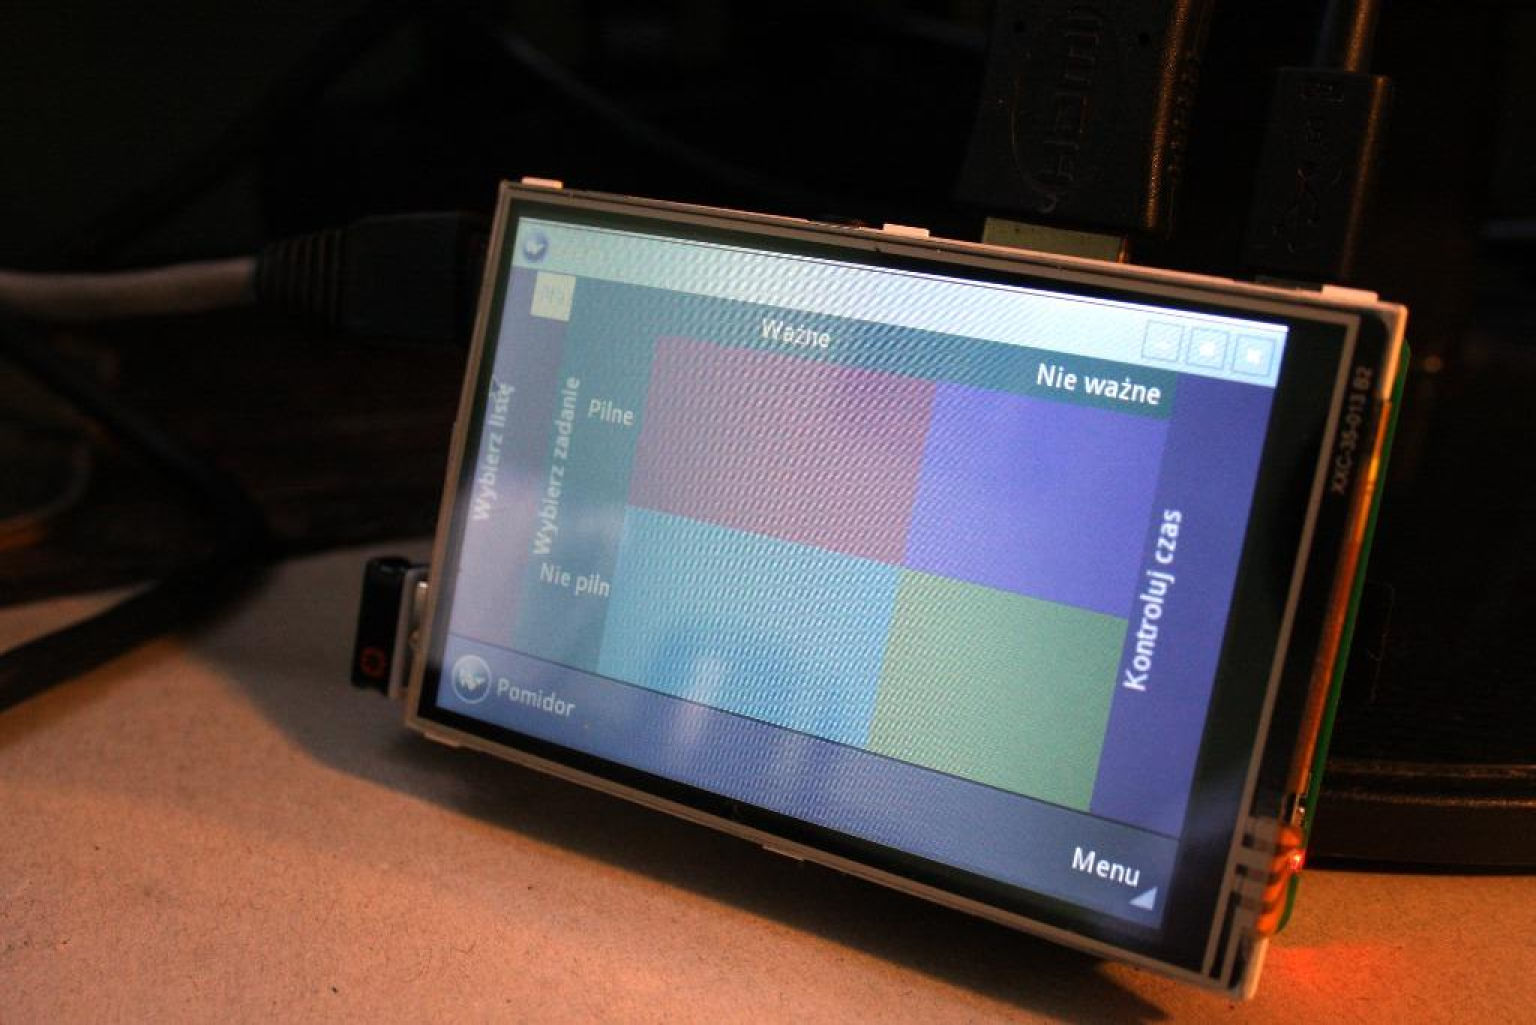
\includegraphics[width=\textwidth]{images/przyklad.png}
  \caption{Aplikacja zainstalowana na urządzeniu}
  \label{figure:przykladowa_app}
\end{figure}
